\begin{frame}
  \begin{block}{Processo de validação}
    \begin{itemize}
      \item Necessário para a validação do modelo proposto
      \item Mudanças de cenários
      \begin{itemize}
        \item Mudanças nas chegadas
        \item Tempos de serviços
        \item Número de usuários
        \item Custos
      \end{itemize}
      \item Três cenários foram propostos: \alert{SCEN1}, \alert{SCEN2} e \alert{SCEN3}
      \item Em todos os parâmetros de rede foram mantidos  
      \item Alterações realizadas nos custos dos atributos que devem ser minimizados
    \end{itemize}
  \end{block}
\end{frame}

\begin{frame}
  \begin{block}
    \begin{itemize}
      \item Na tabela III estão presentes os parametros utilizados nos cenários
      \item 
    \end{itemize}
  \end{block}
  \begin{figure}
    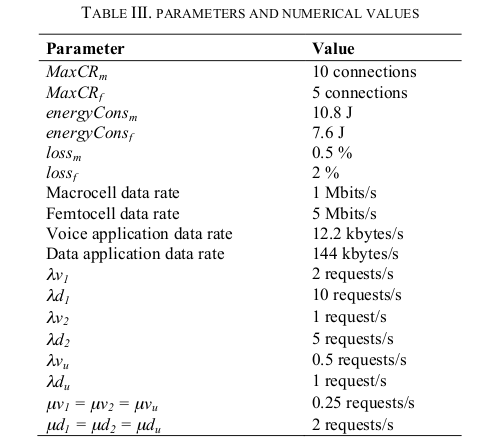
\includegraphics [scale=1.4]{./Figures/table3}
  \end{figure}
\end{frame}
%\begin{frame}
%  \begin{block}{}
%    \begin{itemize}
%      \item
%    \end{itemize}
%  \end{block}
%\end{frame}

%\begin{frame}
%  \begin{block}{}
%  \end{block}
%\end{frame}

%\begin{frame}
%  \begin{figure}[h]
%  	\begin{center}
%      \includegraphics [scale=0.3]{./Figures/Device-Estimates}
%     % \caption {Estimativa de dispositivos conectados à Internet.}
%  		%\label{fig:arq-imuno}
%  	\end{center}
%  \end{figure}
%\end{frame}

%\begin{frame}{Redes de Acesso}
%	\begin{figure}[!htb]
%		\centering
%		\subfloat[DSL]{
%			\includegraphics[height=3.5cm]{./Figures/DSLaccess}
%			\label{figdroopy}}
%		\quad %espaco separador
%		\subfloat[Cable]{
%			\includegraphics[height=3.5cm]{./Figures/CableAccess}
%			\label{figsnoop}}
%		%\caption{Subfiguras}
%		%\label{fig01}
%	\end{figure}
%\end{frame}

%\begin{frame}[fragile]
%\scriptsize
%\begin{verbatim}
%\end{verbatim}
%\end{frame}
